\section{Erweiterung des Squarify Algorithmus} \label{sec:VerbesserungSquarify}
In diesem Abschnitt wird der Squarify Algorithmus \cite{bruls2000squarified}, wie er in Abschnitt \ref{sec:Squarify} beschrieben wurde, auf verschiedene Weisen erweitert und angepasst, um das Layoutproblem, wie es in Abschnitt \ref{sec:TreemapProblem} beschrieben wurde, anzugehen. 

\subsection{Approximative Fläche} \label{sec:ApproxFläche}
Die Grundlegende Idee dieser Erweiterung ist es, die Fläche der Knoten plus die Benötigte Fläche für die Abstände vor berechnung des Layouts zu approximieren.

Dafür brauche ich erstmal einen guten Algorithmus der das Layout gut macht, dann kann ich mit KI die Fläche lernen. Ist die frage ob das wirklich so gut funktionieren kann.

Problem man kann sich sehr gut beispiele konstuieren, bei denen das nicth funktionieren wird. Man kann das natürlich mit skalierung wieder lösen, aber das ist natürlich nicht optimal.

\subsection{Zweifache Berechnung} \label{sec:ZweifachBerechnung}
Die Grundlegende Idee dieser Erweiterung ist es, dass sich die Fläche der Knoten mit Abstand durch das Layout und die Fläche der Knoten ohne Abstand approximieren lässt. Die Idee ist es also einen ersten Durchlauf zu machen, bei dem das Layout ohne Abstand berechnet wird. Dann werden die Größen der Knoten entsprechend dem Layout angepasst, sodass die Größe der Knoten nun auch den Abstand berücksichtigt. Anschließend wird ein zweiter Durchlauf mit diesen angepassten Größen durchgeführt, um das finale Layout zu berechnen.

Bevor wir uns die Details und Ergebnisse dieser Erweiterung anschauen, wollen wir vorweg nehmen, dass diese Erweitung natürlich nicht optimal funktionieren kann und das auch klar ist, da sich die die Änderung der Größe der Knoten natürlich auch das Layout im Zeweiten Durchlauf ändern wird, wodurch die Größen der Knoten wieder nicht korrekt sind. Was ja überhaupt erst das Grundlegende Problem ist (siehe Abshnictt \ref{sec:Problemstellung}). Allerdings ist es ein erster Schritt sich dem Problem zu nähern und zu schauen, ob es sich lohnt in diese Richtung weiter zu forschen.

Der Grundlegende Algorithmus bleibt also (fast) gleich, nur dass zwischen dem ersten und dem zweiten Durchlauf ein zusätzlicher Schritt \textit{Größenanpassung} eingefügt wird. Die Einzige änderung die vorgenommen werden muss ist, dass Knoten nur mit dem definierten Abstand zwischen dem Elternknoten platziert werden können und generell die Fläche des Elternknotens um den Abstand verkleinert wird.
Außerdem ist es nötig nach dem zweiten Durchlauf die Knoten, deren größenwert ja nun den abstand beinhalten, zu verkleinern, um auch den abstand zwischen den Geschwistern herzustellen. Es ist zu erkennen, dass dadurch der Abstand sowohl zwischen Geschwistern als auch zu den Elternknoten den doppelten wert des definierten Abstands hat, dieses Problem ignorieren wir hier, da man es trivialierweise lösen könnte, indem man immer nur die hälfte des Abstands zwischen Geschwistern und Elternknoten abzieht, was wir hier der einfachheit halber nicht tun. -- ODER VIELLEICHT HIER IN DER THESIS DOCH? DANN KÖNNTE ICH MIR DIESEN ABSCHNITT SPAREN, AUCH WENN ES IN DER IMPLEMENTIERUNG AM ENDE ANDERS IST

Wir stellen verschiedene Ansätze vor, was sowohl die Größenanpassung als auch die Anpassung der Knoten nach dem zweiten Durchlauf angeht.
Die Algorithmen funktionieren allerdings alle nach ähnlichem Prinzip: Es wird zunächst für jeden Knoten die Fläche die der Abstand in diesem Layout benötigen würde addiert, indem die Fläche aus der neuen Länge (alte Länge + 2 mal den Abstand) und der neuen Breite (alte Breite + 2 mal den Abstand) berechnet wird. Zusätzlich wird für Elternknoten die Flächenvergrößerung aller Kindernkoten addiert. An dieser Stelle ist allerdings nicht klar, wie sich die Flächenvergrößerung der Kinderknoten auf die Fläche der Elternknoten auswirkt, da diese Änderung selbst von der Anordnung der Kinderknoten abhängt. Wir testen verschiedene Ansätze, um die Flächenänderung der Elternknoten in Abhängikeit zu der Flächenänderung der Kinderknoten zu approximieren.

Nach dem zweiten Durchlauf wird nun die Fläche der Knoten so reduziert, dass sowohl der Abstand zwischen Geschwistern als auch der Abstand zu den Elternknoten den gewünschten Wert hat. Dies ist straight forward und wird hier nicht weiter erläutert. Anzumerken ist aber das dieser Schritt speziell abhängt von der Art der Größenanpassung, die im ersten Schritt durchgeführt wurde.

\subsubsection{Einfache Größenanpassung}
Dies ist die einfachste naive Version der Größenanpassung, der Algorithmus zeigt aber gut die zuvor beschriebenen Probleme auf. Die Fläche der Knoten wird um den Abstand in beiden Richtungen vergrößert. Zusätzlich wird die Fläche der Elternknoten um die Fläche der Kinderknoten vergrößert. 

\begin{algorithm}[H]
\caption{Einfache Größenanpassung}
\label{alg:EinfacheGrößenanpassung}
\begin{algorithmic}[1]
\Function{increaseValuesSimple}{node: SquarifyNode, margin: number}
    \State childrenValueIncrease $\gets$ 0
    \If{node.children}
        \For{child in node.children}
            \State childrenValueIncrease += increaseValuesSimple(child, margin)
        \EndFor
    \EndIf
    \State valueIncrease $\gets$ width * margin * 2 + length * margin * 2 + margin * margin * 4 + childrenValueIncrease
    \State node.value += valueIncrease
    \State \Return valueIncrease
\EndFunction
\end{algorithmic}
\end{algorithm}

Das Problem des Algorithmuses ist am besten an einem Beispiel zu verdeutlichen. Wir visualieren den ZWITEN AnHANG - auch wieder eine händisch erstellte Map, um das Problem zu verdeutlichen. In Abbildung \ref{fig:zeroMarginSquarifyArtifialTwo} ist das Layout mit einem Abstand von 0 zu sehen. 

\begin{figure}
    \centering
    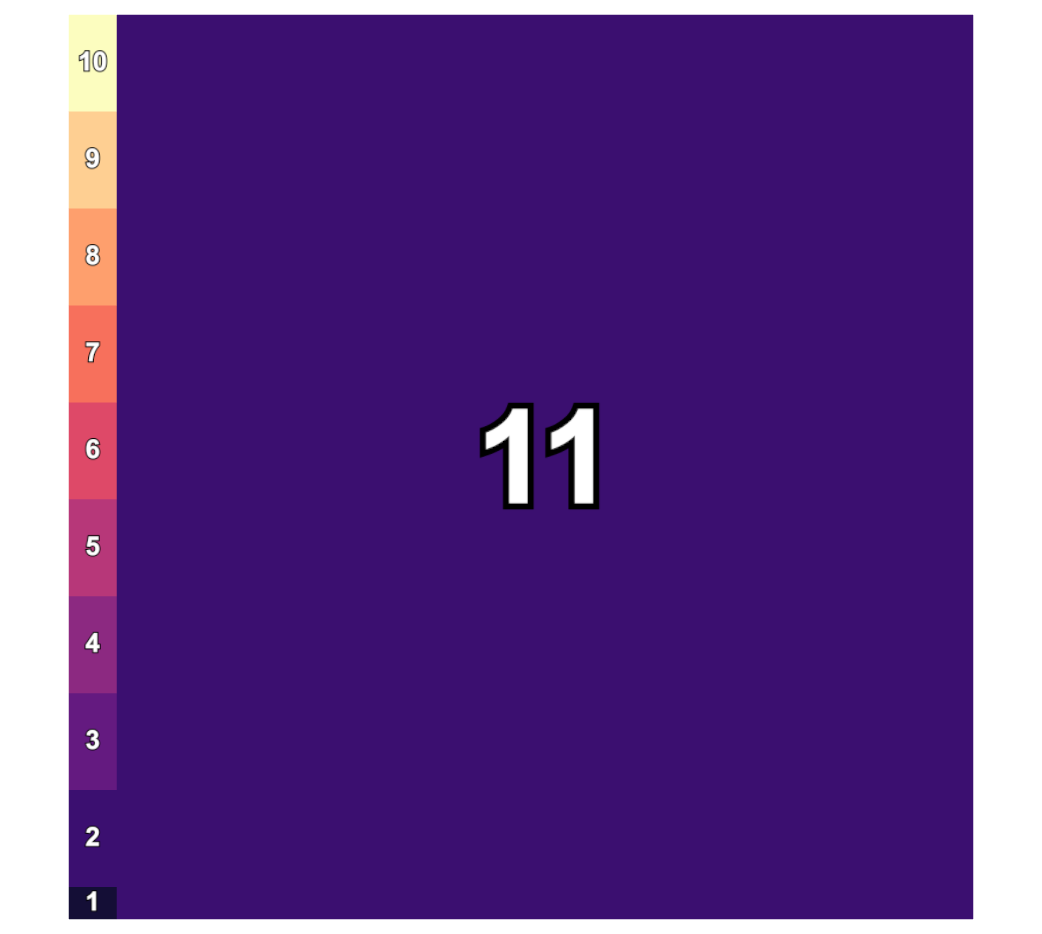
\includegraphics[width=0.8\textwidth]{images/zeroMarginSquarifyArtifialTwo.png}
    \caption{Treemap Layout generiert mit dem Squarify Algorithmus nach Abschnitt \ref{sec:Squarify} mit einem Abstand von 0 und der einfachen Größenanpassung auf der händisch erstellen map (siehe Anhang).}
    \label{fig:zeroMarginSquarifyArtifialTwo}
\end{figure}

In Abbildung \ref{fig:simpleIncreaseMarginOne} ist das Layout mit einem Abstand von 1 zu sehen. Es ist zu erkennen, dass die Knoten auf der linken Seite des Layouts sich außerhalb ihrer Elternknoten erstrecken. Warum passiert das? Knoten 10 ist im zweiten Layout-Schritt deutlich schmaler als im ersten Layout-Schritt. Dadurch wird die Fläche die durch den Abstand eingenommen wird größer als angenommen, weshalb die Fläche des Knotens nach abzug des Abstands im letzen Schritt kleiner ist, als gewünscht. Dementsprechend ist auch die Fläche der Knoten unten links größer als gewünscht, da das Layout der Knoten im zweiten Layout-Schritt quadratischer wird. Knoten 5, der Knoten, der am Quadratischsten ist, wird also am größten erscheinen. Obwohl beide den selben wert haben ist Knoten 5 ca. 1,2 mal größer als Knoten 10) In diesem Beispiel erscheint der unterschied kaum merklich, aber es gibt ihn trotzdem und in anderen fällen kann dieser Unterschied merklich werden.
Viel signifikanter ist aber der Effekt, dass Elternknoten ebenfalls immer schmaler werden, wodurch die fläche, die der innerere abstand einnimm, ebenfalls größer wird und dass sogar immer mehr von ebene zu ebene, wenn man runter geht. Dadurch wird die Fläche für die Kindknoten immer kleiner, was dazu führt, dass Knoten teilweise über ihre Elternknoten hinauswachsen.

\begin{figure}
    \centering
    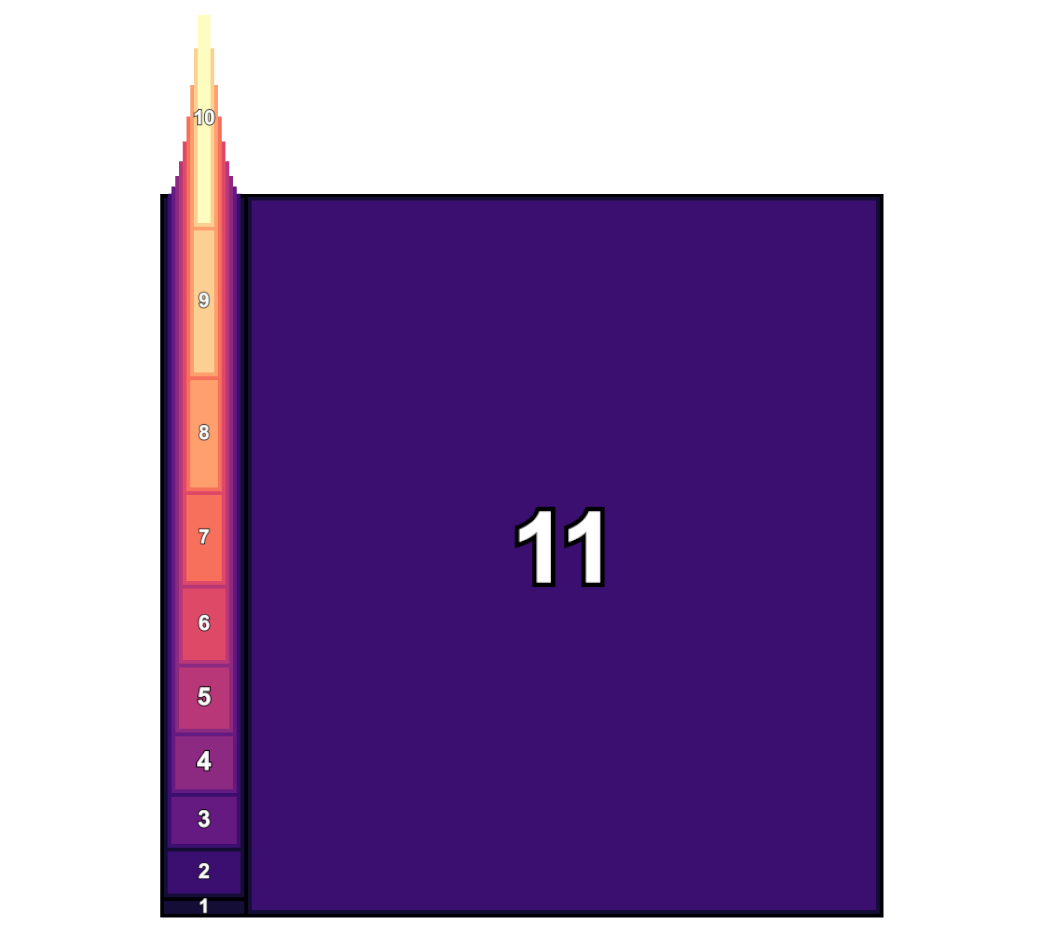
\includegraphics[width=0.8\textwidth]{images/simpleIncreaseMarginOne.png}
    \caption{Treemap Layout generiert mit dem Squarify Algorithmus nach Abschnitt \ref{sec:Squarify} mit einem Abstand von 1 und der einfachen Größenanpassung auf der händisch erstellen map (siehe Anhang).}
    \label{fig:simpleIncreaseMarginOne}
\end{figure}

Dieser Effekt kann einfach behoben werden, wie wir in Abschnitt \ref{sec:ScalingKnoten} sehen werden.

\subsubsection{Relative Größenanpassung}
Bei der berechnung zuvor wurde einfach der margin fläche eines Elternknotens berechnet, auf basis der alten Fläche, ohne die Flächenädnerung durch die Kinderknoten zu berücksichtigen. dadurch wird die resultierende Fläche der Elternknoten zu klein sein, da die Fläche der Kinderknoten nicht berücksichtigt wird.
Die Idee bei dieser Erweiterung ist es die Änderung der Kinder schon vor dem Hinzufügen der Abstandsfläche zu berücksichtigen. Dafür muss die relative Flächenänderung durch die Kindknoten berechnet werden. und damit dann die Seitenlängen anpassen und dann die margins hinzufügen, um die neue Fläche zu erhalten.
Der Algorthmus wird im foldenden als Pseudocode dargestellt (siehe Algorithmus \ref{alg:ZweifachBerechnung}). 

\begin{algorithm}[H]
\caption{Relative Größenanpassung}
\label{alg:ZweifachBerechnung}
\begin{algorithmic}[1]
\Function{increaseValues}{node: SquarifyNode, margin: number}
    \State childrenValueIncrease $\gets$ 0
    \If{node.children}
        \For{child in node.children}
            \State childrenValueIncrease += increaseValues(child, margin)
        \EndFor
    \EndIf

    \State ratioChildrenValueIncrease $\gets$ (node.value + childrenValueIncrease) / node.value

    \State valueIncrease $\gets$ 
        Math.sqrt(ratioChildrenValueIncrease) * width * margin * 2 +
        Math.sqrt(ratioChildrenValueIncrease) * length * margin * 2 +
        margin * margin * 4 +
        childrenValueIncrease

    \State node.value += valueIncrease
    \State \Return valueIncrease
\EndFunction
\end{algorithmic}
\end{algorithm}

Problem:
Der Algorithmus in dieser Form zeigt einige Probleme auf. Die Flächenvergrößerung der Kindknoten sagt nichts darüber aus, in welche Richtung sich die Fläche ändert. Es wird davon ausgegangen, dass sich die Fläche gleichmäßig in beide Richtungen ändert (siehe Zeile 13 und 14 in Algorithmus ZEILEN ANPASSEN  \ref{alg:ZweifachBerechnung}). 
es kommt also zu ähnlichen Problem wie davor. es können knoten sowohl zu viel platz als auch zu wenig Platz bekommen, jenachdem ob Sie im zweiten schritt quadratischer oder schmaler werden.  Siehe Abbildung \ref{fig:relativeIncreaseMarginOne} für ein Beispiel.

\begin{figure}
    \centering
    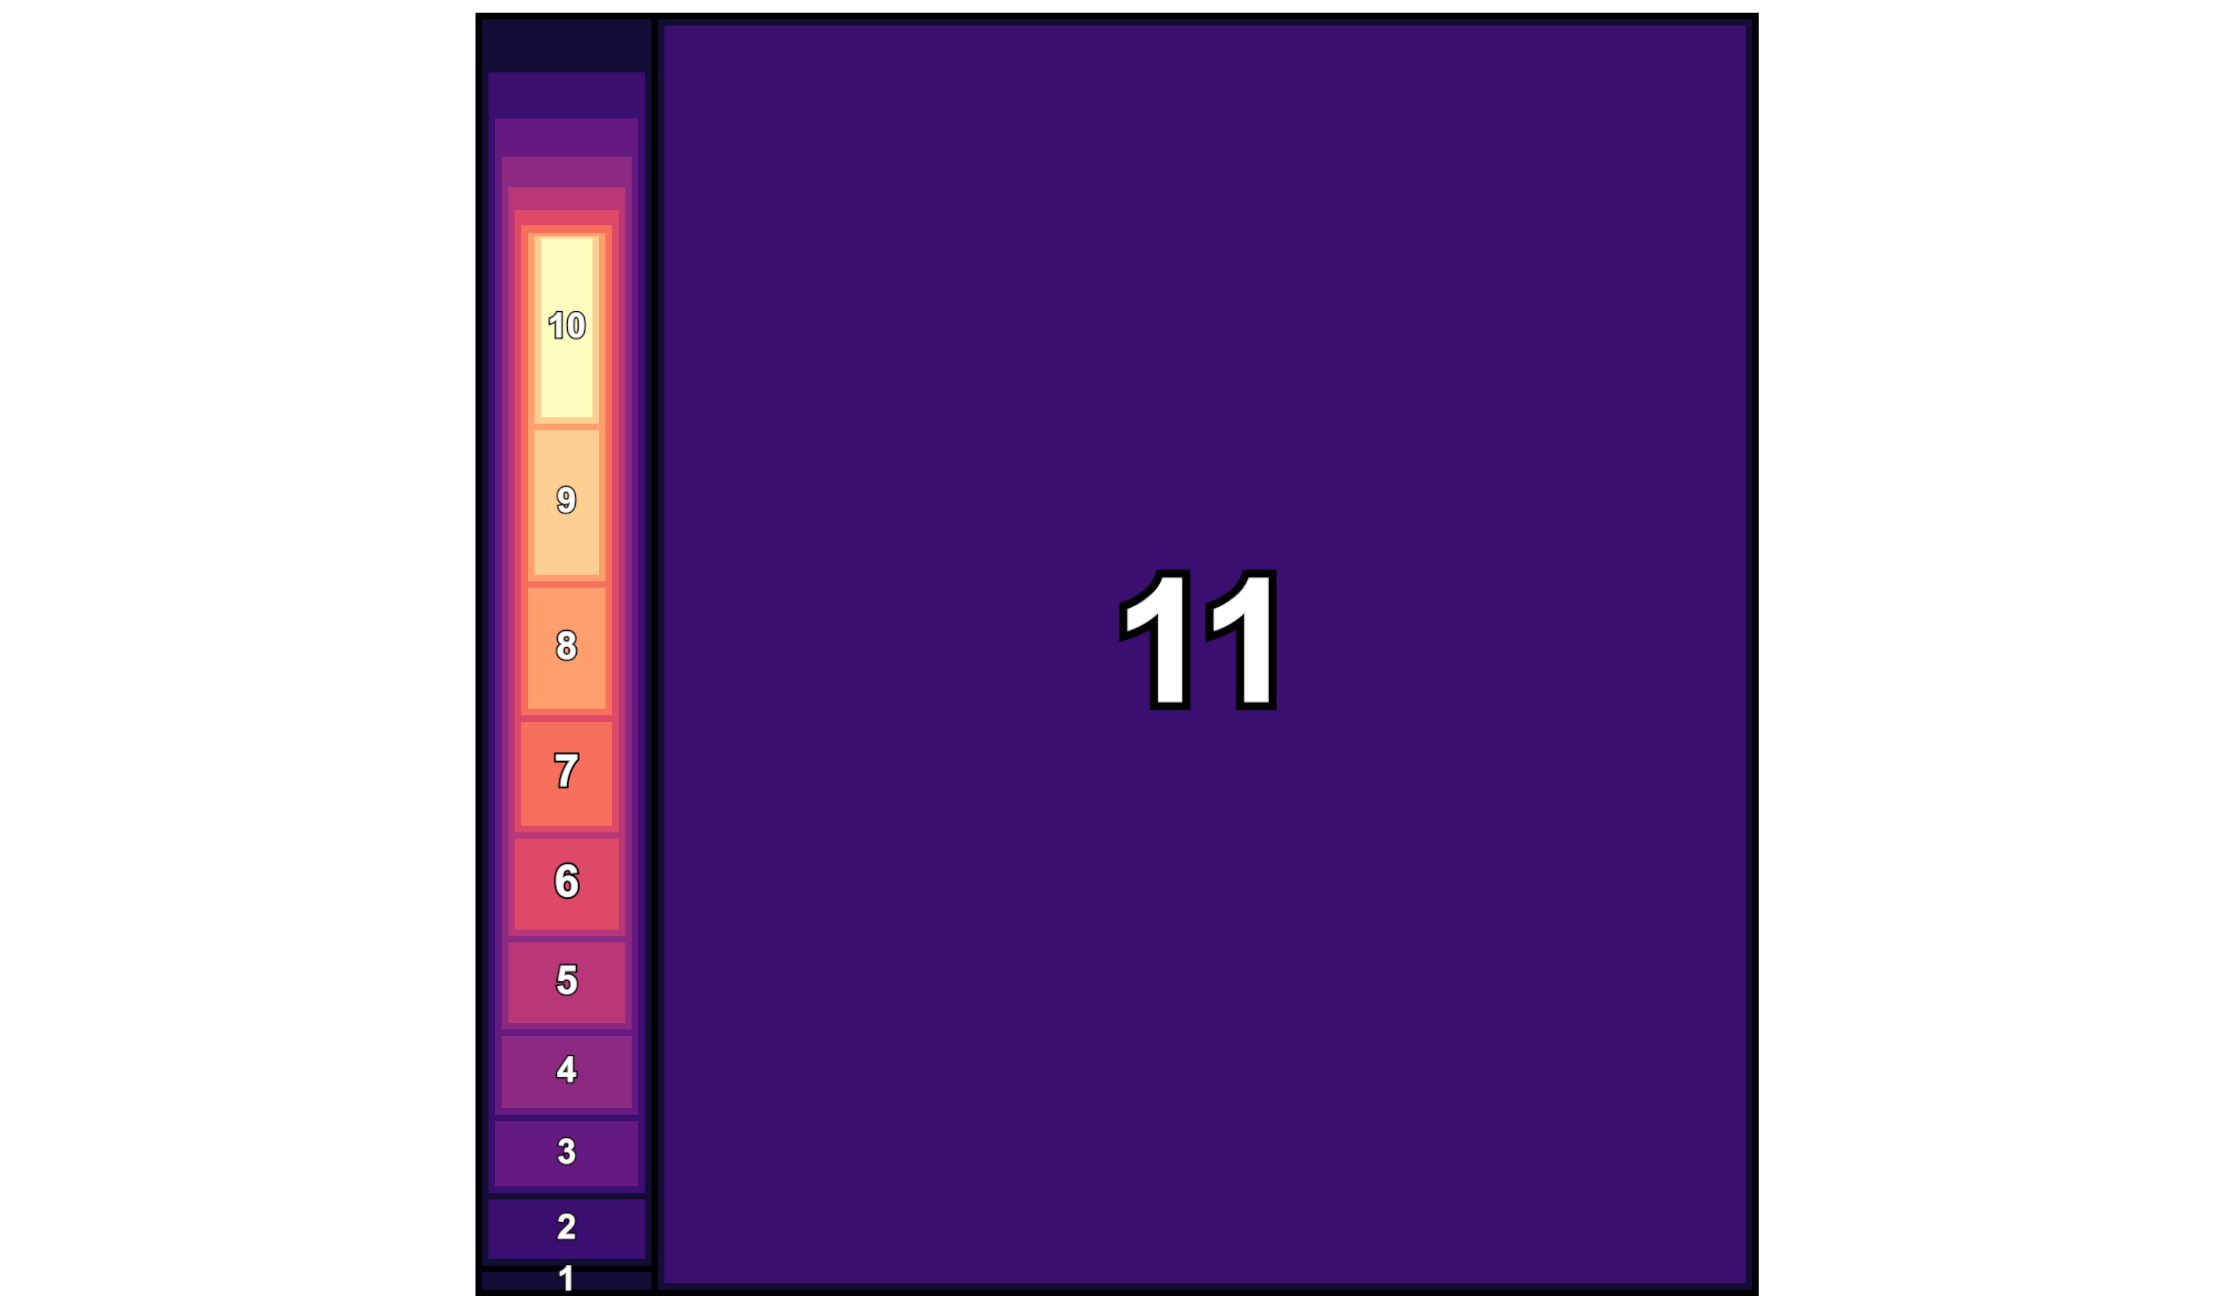
\includegraphics[width=0.8\textwidth]{images/increaseMarginOne.png}
    \caption{Treemap Layout generiert mit dem Squarify Algorithmus nach Abschnitt \ref{sec:Squarify} mit einem Abstand von 1 und der relativen Größenanpassung auf der händisch erstellen map (siehe Anhang).}
    \label{fig:relativeIncreaseMarginOne}
\end{figure}

\subsection{Scaling der Knoten} \label{sec:ScalingKnoten}
Wenn die Fläche innnerhalb von Elternknoten immer kleiner wird, kann es passieren, dass Knoten über ihre Elternknoten hinauswachsen, wie in Abbildung \ref{fig:simpleIncreaseMarginOne} zu sehen ist. Es kann genauso passieren, dass die Fläche innerhalb der Knoten größer wird, wie in Abbildung \ref{fig:relativeIncreaseMarginOne} auf der linken seite zu erkennen ist. Dieser Effekt kann trivialer weise behoben werden, indem der zweite Layout-Schritt angepasst wird, sodass die Knoten immer auf die Fläche des Elternknotens skaliert werden. 
Vor jeden Squarify-Schritt wird dafür die wirklich zur verfügung stehende Fläche des Elternknotens berechnet und die Kindknoten entsprechend dieser Änderung skaliert, sodass sie genau in die Fläche des Elternknotens passen.

Der Nachteil dieser Methode ist in Abbildung \ref{fig:simpleIncreaseMarginOneScale} zu erkennen. Die Knoten werden dadurch natürlich nicht mehr proportional zu ihren Werten sein. Knoten 10 hat zum beispiel ein Verhältnis von ca. 0.5 zu seinem Wert, während Knoten 6 ein Verhältnis von ca. 1.4 zu seinem Wert hat.

\begin{figure}
    \centering
    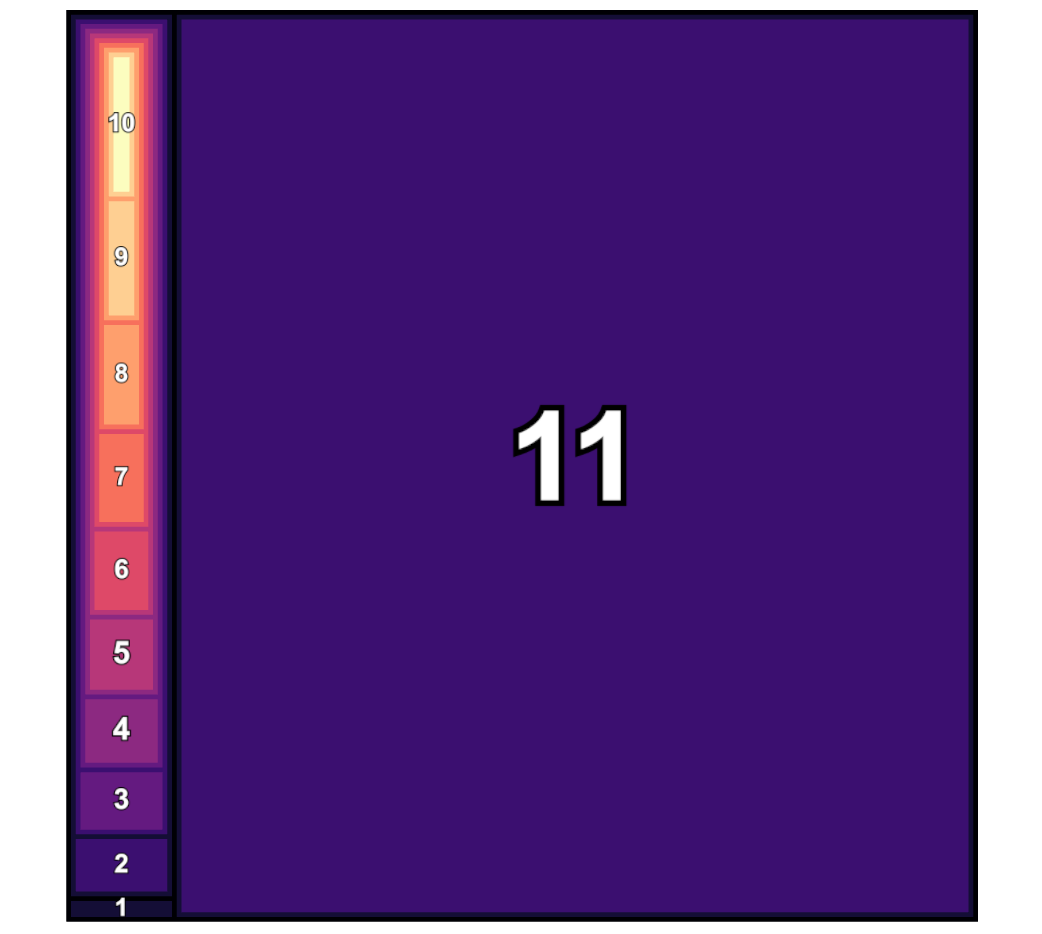
\includegraphics[width=0.8\textwidth]{images/simpleIncreaseMarginOneScale.png}
    \caption{Treemap Layout generiert mit dem Squarify Algorithmus nach Abschnitt \ref{sec:Squarify} mit einem Abstand von 1 und der einfachen Größenanpassung auf der händisch erstellen map (siehe Anhang) und der Skalierung der Knoten.}
    \label{fig:simpleIncreaseMarginOneScale}
\end{figure}

Je genauer die Größenanpassung der Knoten ist, desto geringer fällt natürlich dieser Effekt aus. Siehe im Vergleich dazu Abbildung \ref{fig:relativeIncreaseMarginOneScale}, da die relative Größenanpassung deutlich genauer ist, ist der Effekt hier auch deutlich geringer. Knoten 10 hat Größe 40 und Knoten 6 hat Größe 41, was fast ähnlich Groß ist.

\begin{figure}
    \centering
    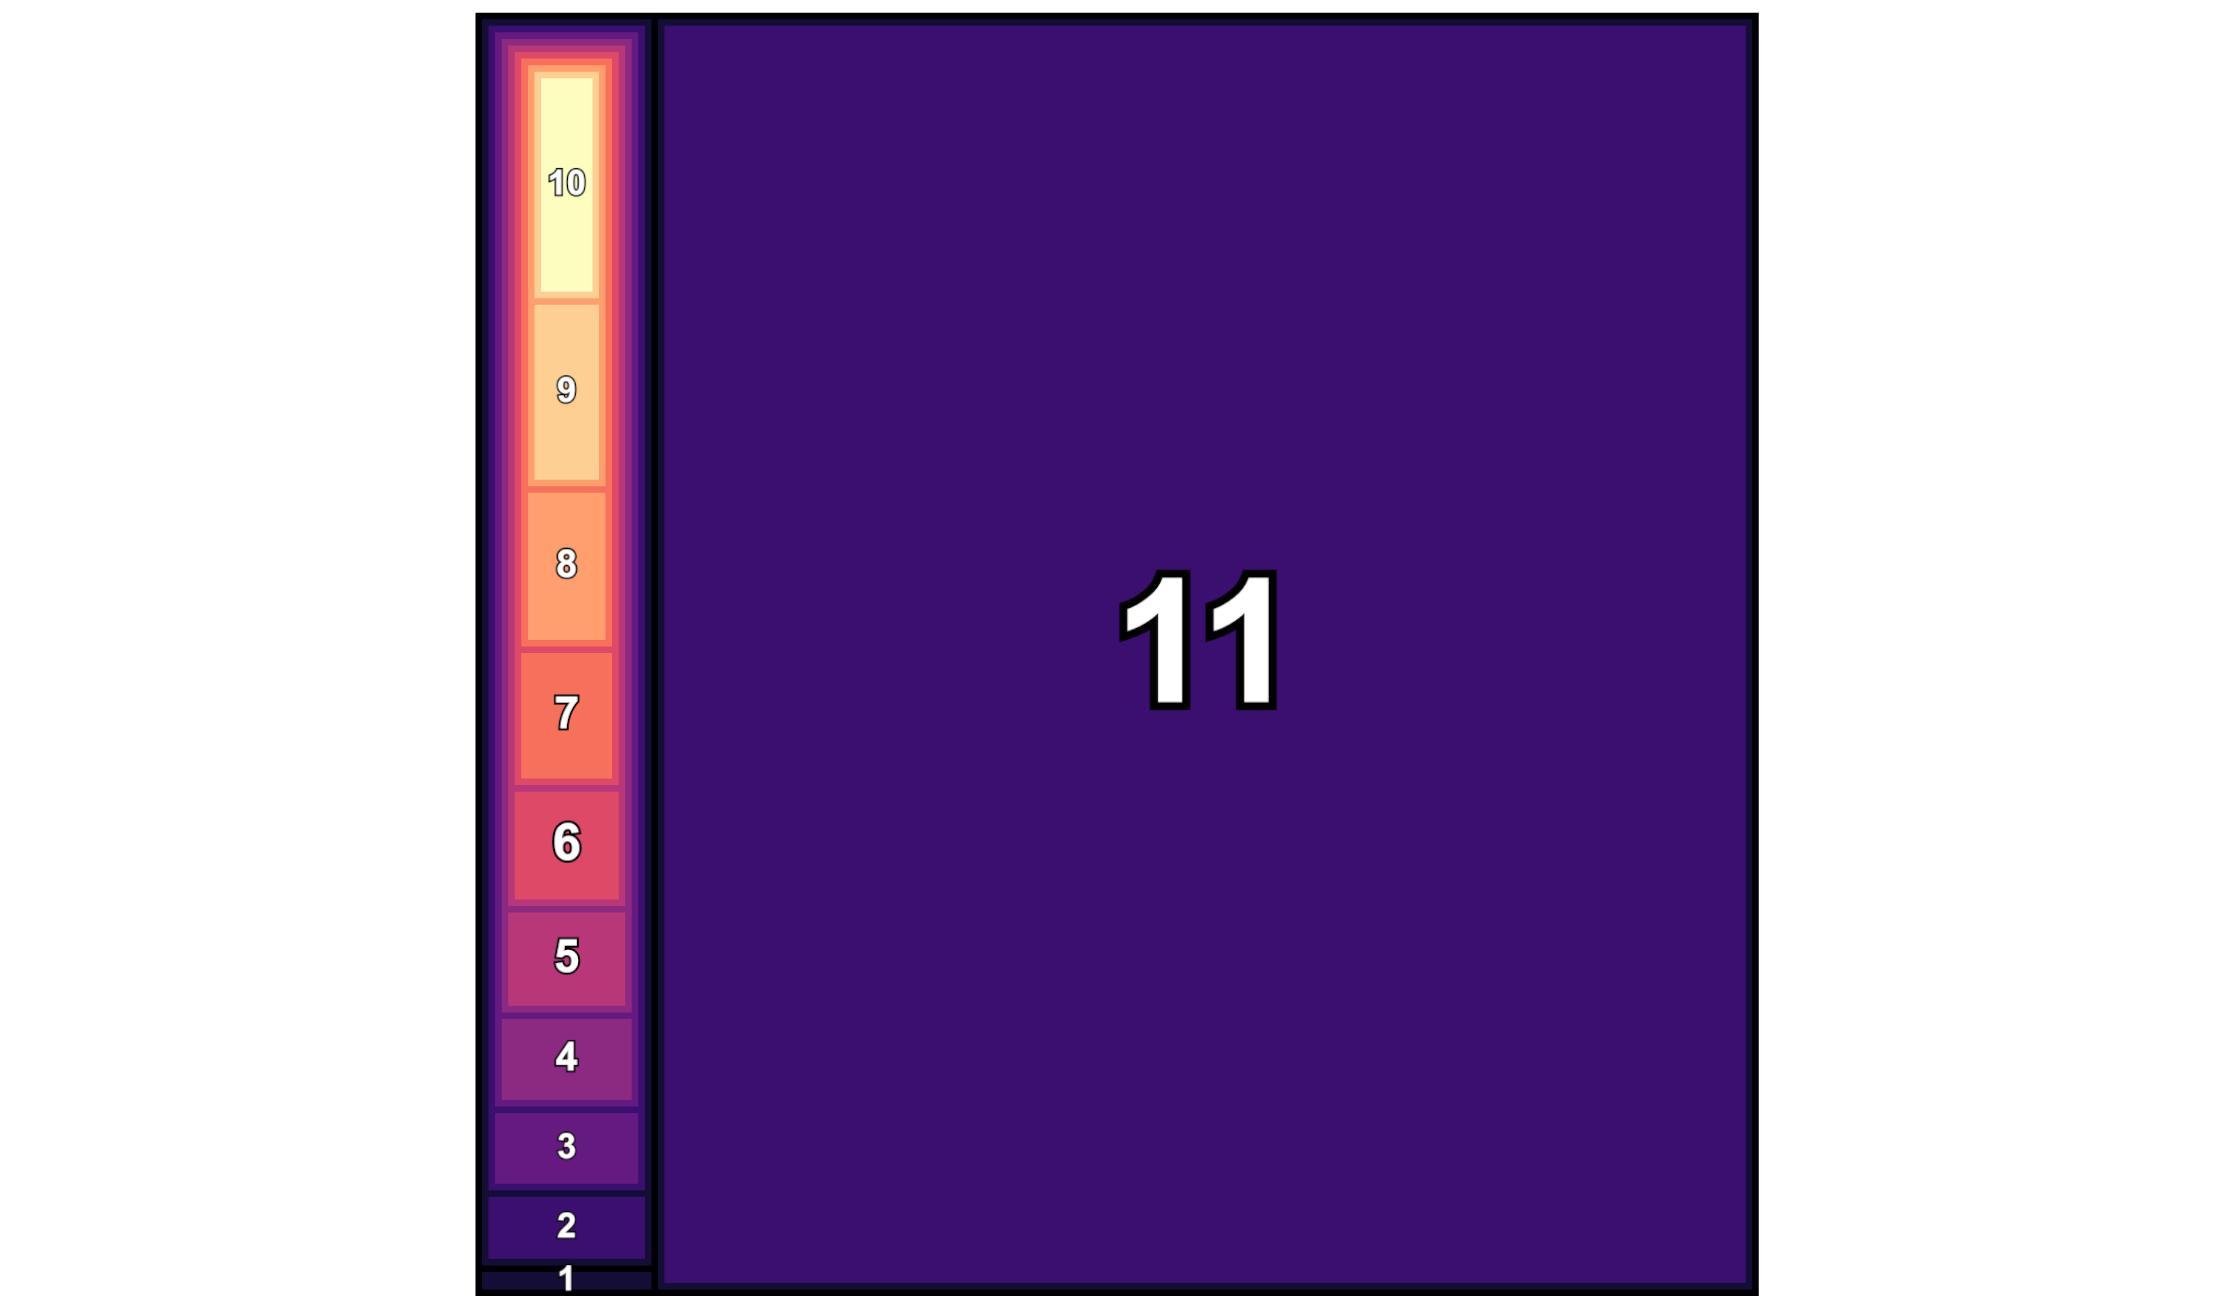
\includegraphics[width=0.8\textwidth]{images/increaseMarginOneScale.png}
    \caption{Treemap Layout generiert mit dem Squarify Algorithmus nach Abschnitt \ref{sec:Squarify} mit einem Abstand von 1 und der relativen Größenanpassung auf der händisch erstellen map (siehe Anhang) und der Skalierung der Knoten.}
    \label{fig:relativeIncreaseMarginOneScale}
\end{figure}

Persönlich würde ich sagen, dass dieser Effekt für das herunter skalieren der Knoten gut ist, da sonst eine grundlegende eigenschaft der Darstellung verletzt wird, aber für das hoch skalieren der Knoten könnte man auch sagen, dass es wichtiger ist die Fläche der Knoten proportional zu ihren Werten zu halten, als die \textit{verschwendete} Fläche aufzufüllen. Diese jetzt hier sehr subjektive Einschätzung wird aber nochmal genauer beläuchtet in der evaluation und vergleich.

\subsection{Reihenfolge der Knoten} \label{sec:ReihenfolgeKnoten}
Die Reienfolge in der die knoten in das Layout eingefügt werden, hat einen großen Einfluss auf das Layout. \cite{johnson1991tree} haben in ihrem Paper herausgefunden, dass die ergebnisse am besten sind, wenn die Knoten in der Reihenfolge der Größe eingefügt werden. Also der Größte zuerst.

\subsection{Mehrfache Berechnung} \label{sec:MehrfacheBerechnung}
Die Grundlegende Idee dieser Erweiterung ist es, das Layout mehrfach zu berechnen und dabei die Fläche der Knoten immer weiter anzupassen. Dies wird so lange wiederholt, bis sich die Fläche der Knoten nicht mehr ändert oder eine maximale Anzahl an Iterationen erreicht ist.

\subsection{Anpassung der Knoten}
In bild updateValues.png ist zu erkennen, dass kp. margin 10 noP 3


\subsection{Fazit}
Immernoch straight forward, es gibt aber noch Probleme 

Warum besonders den squarify algorithmus betrachtet und nicht zum beipsiel pivot oder circle?? -> weil diese Andere Ziele haben -> noch mehr begründen anhand der definierten Ziele